\chapter{Testes e Resultados} \label{chap:testsResults}
	\section{Experimento 01}
	\begin{figure}[h]
		\centering
		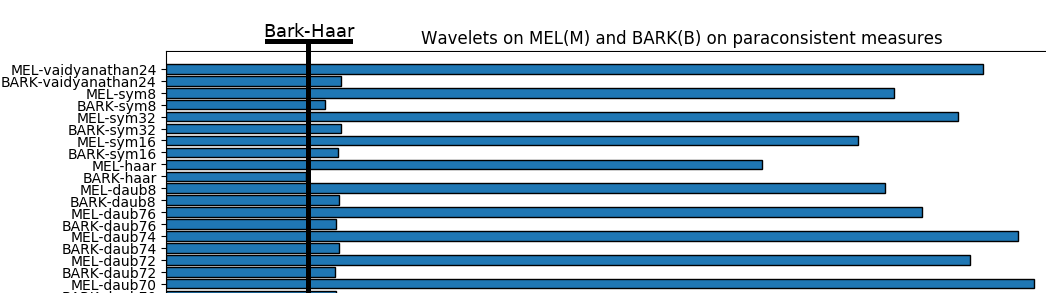
\includegraphics[width=\linewidth]{images/results/paraconsistentPlane/ParaconsistentParcial.png}
		\caption{Distância da combinação Wavelet\textit{X}BARK ou MEL do ponto (1,0)}
		\label{fig:ParaconsistentParcial}
	\end{figure}

	\begin{table}[h]
	\newcommand{\mc}[3]{\multicolumn{#1}{#2}{#3}}
	\definecolor{tcB}{rgb}{0.447059,0.74902,0.266667}
	\definecolor{tcA}{rgb}{0.65098,0.65098,0.65098}
	\definecolor{tcC}{rgb}{1,0.94902,0}
	\begin{center}
		\begin{tabular}{|c|c|c|c|}\hline
			% use packages: color,colortbl
			\rowcolor{tcA}
			Wavelet & G1 & G2 & Distancia do ponto (1,0)\\\hline
			\rowcolor{tcB}
			haar & 0.93615 & 4.68316e-310 & 0.0638503\\\hline
			\mc{1}{|>{\columncolor{tcC}}c|}{daub4} & \mc{1}{>{\columncolor{tcC}}c|}{0.928088} & \mc{1}{>{\columncolor{tcC}}c|}{4.68316e-310} & \mc{1}{>{\columncolor{tcC}}c|}{0.0719123}\\\hline
			\mc{1}{|>{\columncolor{tcC}}c|}{daub6} & \mc{1}{>{\columncolor{tcC}}c|}{0.927885} & \mc{1}{>{\columncolor{tcC}}c|}{4.68316e-310} & \mc{1}{>{\columncolor{tcC}}c|}{0.072115}\\\hline
			\mc{1}{|>{\columncolor{tcC}}c|}{coif6} & \mc{1}{>{\columncolor{tcC}}c|}{0.927823} & \mc{1}{>{\columncolor{tcC}}c|}{4.68316e-310} & \mc{1}{>{\columncolor{tcC}}c|}{0.072177}\\\hline
			\mc{1}{|>{\columncolor{tcC}}c|}{sym8} & \mc{1}{>{\columncolor{tcC}}c|}{0.92769} & \mc{1}{>{\columncolor{tcC}}c|}{4.68316e-310} & \mc{1}{>{\columncolor{tcC}}c|}{0.0723096}\\\hline
			\mc{1}{|>{\columncolor{tcC}}c|}{daub12} & \mc{1}{>{\columncolor{tcC}}c|}{0.926541} & \mc{1}{>{\columncolor{tcC}}c|}{4.68316e-310} & \mc{1}{>{\columncolor{tcC}}c|}{0.073459}\\\hline
		\end{tabular}
	\end{center}
	\caption{Wavelet\textit{X}BARK no plano paraconsistente}
	\label{tab:distParacomBest}
\end{table}

	\par Na figura \ref{fig:ParaconsistentParcial} quanto menor o valor, mais disjuntos tendem ser os vetores de características gerados para as duas classes testadas (\textit{spoofing }e não \textit{spoofing}). Como se pode constatar, das combinações testadas, a \textit{\textbf{Haar com BARK}} conseguiu o \textbf{melhor desempenho} na criação dos melhores vetores de características. A tabela \ref{tab:distParacomBest} mostra os 6 melhores resultados em distância do ponto (1,0)(verdade) no plano paraconsistente, a totalidade dos dados se encontram no apêndice deste documento nas tabelas \ref{tab:distParacomFrom10Bark_1} e \ref{tab:distParacomFrom10Bark_2} para todos os resultados com BARK e nas tabelas \ref{tab:distParacomFrom10Mel_1} e \ref{tab:distParacomFrom10Mel_2} para os com MEL. Na figura \ref{fig:paraconsistentfull} se pode ver o gráfico de barras para todas as combinações \textit{wavelets}X\textit{BARK/MEL}.
	
	\par A combinação \textbf{\textit{wavelet + BARK}} teve, consistentemente, um desempenho \textbf{melhor} do que as respectivas combinações \textbf{\textit{wavelet + MEL}}.
	
	\newpage
	\section{Experimento 02}
		\par Considerando que o experimento 1 teve como melhor resultado a combinação \textbf{Haar+BARK} o objetivo deste é constatar a máxima acurácia que se consegue atingir em um classificador baseado em distâncias Euclidianas e Manhattan. O dimensionamento do tamanho das amostras de referência que neste caso são os itens usados para o treinamento do classificador variou em 10\%, 20\%, 30\%, 40\% e finalmente 50\% do total das amostras. 300 foi a quantidade máxima de testes escolhida.
		\par Os resultados gerais são mostrados na tabela \ref{tab:experiment02ResultsEuclidian} para distância Euclidiana e na tabela \ref{tab:experiment02ResultsManhattan} para distância Manhattan. 
		
		\par Mais níveis de detalhes para a distância Euclidiana pode ser conseguido consultando-se as tabelas \ref{tab:classifier_Euclidian_10}, \ref{tab:classifier_Euclidian_20}, \ref{tab:classifier_Euclidian_30}, \ref{tab:classifier_Euclidian_40},  \ref{tab:classifier_Euclidian_50} e seus respectivos gráficos \ref{fig:classifiereuclidian10}, \ref{fig:classifiereuclidian20}, \ref{fig:classifiereuclidian30}, \ref{fig:classifiereuclidian40}, \ref{fig:classifiereuclidian50}.
		
		\par E para a distância Manhattan podem ser consultadas as tabelas 	\ref{tab:classifier_Manhattan_10}, \ref{tab:classifier_Manhattan_20}, \ref{tab:classifier_Manhattan_30}, \ref{tab:classifier_Manhattan_40}, \ref{tab:classifier_Manhattan_50} e seus respectivos gráficos 		 
		 \ref{fig:classifiermanhattan10}, \ref{fig:classifiermanhattan20}, 	 \ref{fig:classifiermanhattan30}, \ref{fig:classifiermanhattan40},  \ref{fig:classifiermanhattan50}.
			\begin{table}[h]
	\newcommand{\mc}[3]{\multicolumn{#1}{#2}{#3}}
	\definecolor{tcA}{rgb}{0.65098,0.65098,0.65098}
	\definecolor{tcB}{rgb}{0.447059,0.74902,0.266667}
	\begin{center}
		\begin{tabular}{|l|l|l|}\hline
			% use packages: color,colortbl
			\rowcolor{tcA}
			\textbf{Tamanho do modelo} & \textbf{Acurácia mínima} & \textbf{Acurácia máxima}\\\hline
			\rowcolor{tcB}
			\mc{1}{|c|}{10\%} & \mc{1}{c|}{0,6666} & \mc{1}{c|}{0,8861}\\\hline
			\rowcolor{tcB}
			\mc{1}{|c|}{20\%} & \mc{1}{c|}{0,7439} & \mc{1}{c|}{0,8902}\\\hline
			\rowcolor{tcB}
			\mc{1}{|c|}{30\%} & \mc{1}{c|}{0,7665} & \mc{1}{c|}{0,8919}\\\hline
			\rowcolor{tcB}
			\mc{1}{|c|}{40\%} & \mc{1}{c|}{0,7784} & \mc{1}{c|}{0,9024}\\\hline
			\rowcolor{tcB}
			\mc{1}{|c|}{50\%} & \mc{1}{c|}{0,7804} & \mc{1}{c|}{0,9097}\\\hline
		\end{tabular}
	\end{center}
	\caption{Resultados do experimento 02}
	\label{tab:experiment02Results}
\end{table}
			
			\newpage
			\begin{figure}[h]
				\centering
				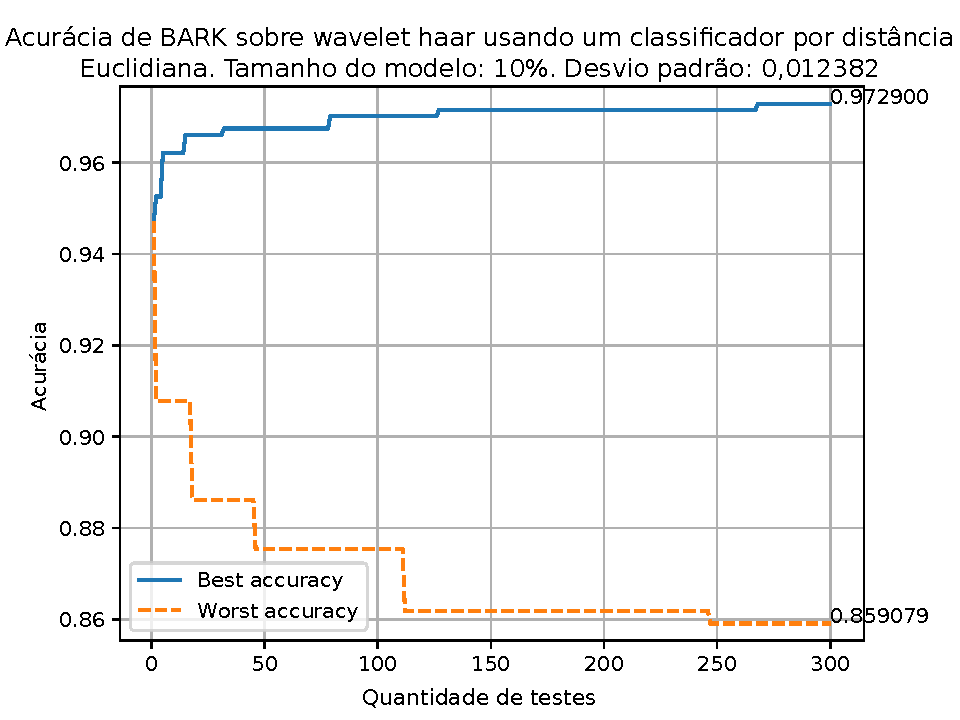
\includegraphics{images/results/confusionMatrices/classifier_Euclidian_10}
				\caption{Acurácia \textit{X} quantidade de testes - Distância Euclidiana, modelo a 10\%}
				\label{fig:classifiereuclidian10}
			\end{figure}
			\begin{table}[H] 					\newcommand{\mc}[3]{\multicolumn{#1}{#2}{#3}} 					\definecolor{tcB}{rgb}{0.447059,0.74902,0.266667} 					\definecolor{tcC}{rgb}{0,0,0} 					\definecolor{tcD}{rgb}{0,0.5,1} 					\definecolor{tcA}{rgb}{0.65098,0.65098,0.65098} 					\begin{center} 						\subfloat[Melhor matriz de confusão]{ 							\begin{tabular}{ccc} 								\mc{1}{l}{} & \mc{1}{>{\columncolor{tcA}}c}{\textbf{genuíno}} & \mc{1}{>{\columncolor{tcA}}c}{\textbf{falseado}}\\ 								\mc{1}{>{\columncolor{tcA}}r}{\textbf{genuíno}} & \mc{1}{>{\columncolor{tcB}}c}{\textcolor{tcC}{363}} & \mc{1}{>{\columncolor{tcD}}c}{\textcolor{tcC}{14}}\\ 								\mc{1}{>{\columncolor{tcA}}r}{\textbf{falseado}} & \mc{1}{>{\columncolor{tcD}}c}{\textcolor{tcC}{6}} & \mc{1}{>{\columncolor{tcB}}c}{\textcolor{tcC}{355}} 							\end{tabular} 							\label{tab:classifier_Euclidian_10_best} 						} 						\qquad 						\subfloat[Pior matriz de confusão]{ 							\begin{tabular}{ccc} 								\mc{1}{l}{} & \mc{1}{>{\columncolor{tcA}}c}{\textbf{genuíno}} & \mc{1}{>{\columncolor{tcA}}c}{\textbf{falseado}}\\ 								\mc{1}{>{\columncolor{tcA}}r}{\textbf{genuíno}} & \mc{1}{>{\columncolor{tcB}}c}{\textcolor{tcC}{275}} & \mc{1}{>{\columncolor{tcD}}c}{\textcolor{tcC}{10}}\\ 								\mc{1}{>{\columncolor{tcA}}r}{\textbf{falseado}} & \mc{1}{>{\columncolor{tcD}}c}{\textcolor{tcC}{94}} & \mc{1}{>{\columncolor{tcB}}c}{\textcolor{tcC}{359}} 							\end{tabular} 							\label{tab:classifier_Euclidian_10_worse} 						} 					\end{center} 					\caption{Matrizes de confusão para distância Euclidiana com modelo a 10\%} 				\end{table}
			\newpage
			\begin{figure}[h]
				\centering
				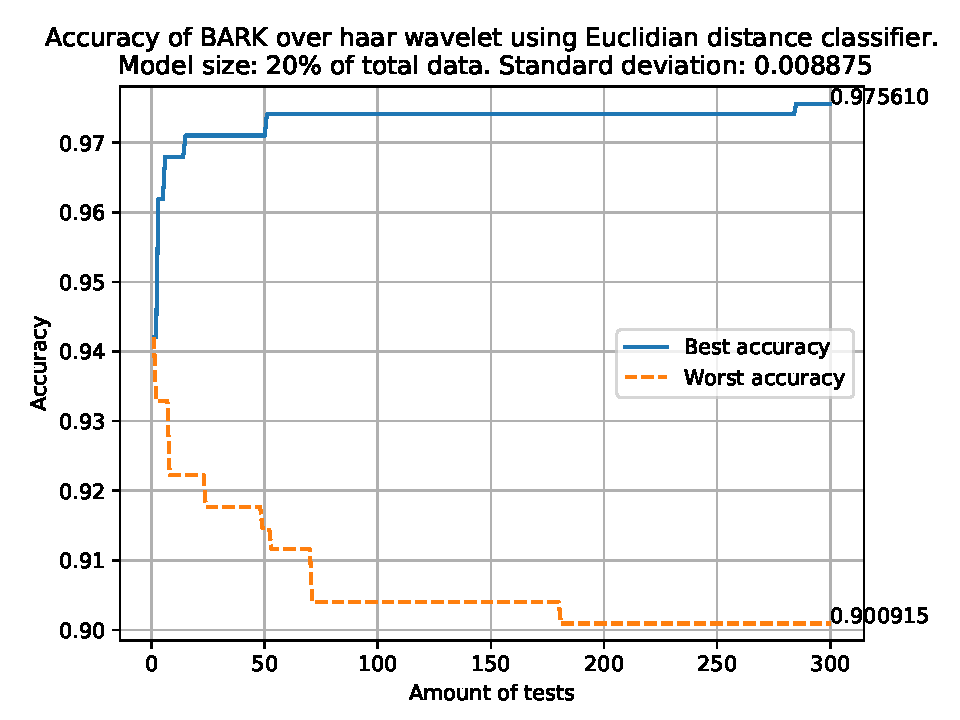
\includegraphics{images/results/confusionMatrices/classifier_Euclidian_20}
				\caption{Acurácia \textit{X} quantidade de testes - Distância Euclidiana, modelo a 20\%}
				\label{fig:classifiereuclidian20}
			\end{figure}
			\begin{table}[h]
\newcommand{\mc}[3]{\multicolumn{#1}{#2}{#3}}
\definecolor{tcB}{rgb}{0.447059,0.74902,0.266667}
\definecolor{tcC}{rgb}{0,0,0}
\definecolor{tcD}{rgb}{0,0.4,0.701961}
\definecolor{tcA}{rgb}{0.65098,0.65098,0.65098}
\begin{center}
	\begin{tabular}{ccc}
		% use packages: color,colortbl
		\mc{1}{l}{} & \mc{1}{>{\columncolor{tcA}}c}{\textbf{genuíno}} & \mc{1}{>{\columncolor{tcA}}c}{\textbf{regravado}}\\

		\mc{1}{>{\columncolor{tcA}}r}{\textbf{genuíno}} & \mc{1}{>{\columncolor{tcB}}c}{\textcolor{tcC}{308}} & \mc{1}{>{\columncolor{tcD}}c}{\textcolor{tcC}{50}}\\

		\mc{1}{>{\columncolor{tcA}}r}{\textbf{regravado}} & \mc{1}{>{\columncolor{tcD}}c}{\textcolor{tcC}{20}} & \mc{1}{>{\columncolor{tcB}}c}{\textcolor{tcC}{278}}
	\end{tabular}
	\caption{Melhor matriz de confusão para o classificador por distâncias Euclidianas com o uso de 20\% da base para modelagem}
	\label{tab:classifier_Euclidian_20_best}
\end{center}
\end{table}

\begin{table}[h]
	\newcommand{\mc}[3]{\multicolumn{#1}{#2}{#3}}
	\definecolor{tcB}{rgb}{0.447059,0.74902,0.266667}
	\definecolor{tcC}{rgb}{0,0,0}
	\definecolor{tcD}{rgb}{0,0.4,0.701961}
	\definecolor{tcA}{rgb}{0.65098,0.65098,0.65098}
	\begin{center}
		\begin{tabular}{ccc}
			% use packages: color,colortbl
			\mc{1}{l}{} & \mc{1}{>{\columncolor{tcA}}c}{\textbf{genuíno}} & \mc{1}{>{\columncolor{tcA}}c}{\textbf{regravado}}\\
			
			\mc{1}{>{\columncolor{tcA}}r}{\textbf{genuíno}} & \mc{1}{>{\columncolor{tcB}}c}{\textcolor{tcC}{295}} & \mc{1}{>{\columncolor{tcD}}c}{\textcolor{tcC}{137}}\\
			
			\mc{1}{>{\columncolor{tcA}}r}{\textbf{regravado}} & \mc{1}{>{\columncolor{tcD}}c}{\textcolor{tcC}{33}} & \mc{1}{>{\columncolor{tcB}}c}{\textcolor{tcC}{191}}
		\end{tabular}
		\caption{Pior matriz de confusão para o classificador por distâncias Euclidianas com o uso de 20\% da base para modelagem}
		\label{tab:classifier_Euclidian_20_worse}
	\end{center}
\end{table}

	
			\newpage
			\begin{figure}[h]
				\centering
				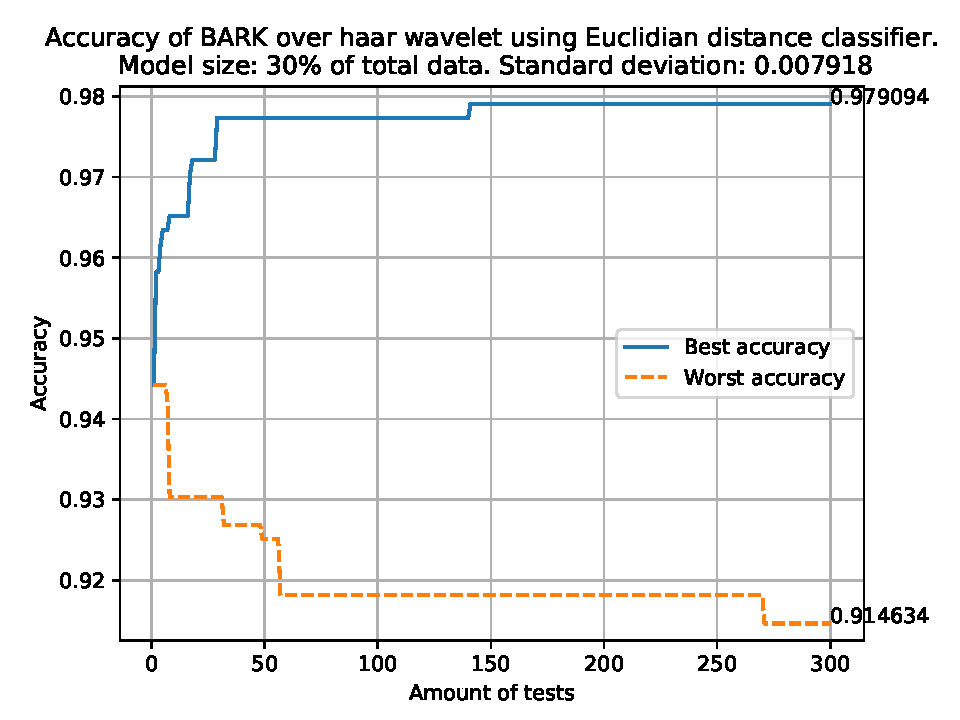
\includegraphics{images/results/confusionMatrices/classifier_Euclidian_30}
				\caption{Acurácia \textit{X} quantidade de testes - Distância Euclidiana, modelo a 30\%}
				\label{fig:classifiereuclidian30}
			\end{figure}
			\begin{table}[H] 					\newcommand{\mc}[3]{\multicolumn{#1}{#2}{#3}} 					\definecolor{tcB}{rgb}{0.447059,0.74902,0.266667} 					\definecolor{tcC}{rgb}{0,0,0} 					\definecolor{tcD}{rgb}{0,0.5,1} 					\definecolor{tcA}{rgb}{0.65098,0.65098,0.65098} 					\begin{center} 		\caption{Matrizes de confusão para distância Euclidiana com modelo a 30\%}				\subfloat[Melhor matriz de confusão]{ 							\begin{tabular}{ccc} 								\mc{1}{l}{} & \mc{1}{>{\columncolor{tcA}}c}{\textbf{genuíno}} & \mc{1}{>{\columncolor{tcA}}c}{\textbf{falseado}}\\ 								\mc{1}{>{\columncolor{tcA}}r}{\textbf{genuíno}} & \mc{1}{>{\columncolor{tcB}}c}{\textcolor{tcC}{283}} & \mc{1}{>{\columncolor{tcD}}c}{\textcolor{tcC}{8}}\\ 								\mc{1}{>{\columncolor{tcA}}r}{\textbf{falseado}} & \mc{1}{>{\columncolor{tcD}}c}{\textcolor{tcC}{4}} & \mc{1}{>{\columncolor{tcB}}c}{\textcolor{tcC}{279}} 							\end{tabular} 							\label{tab:classifier_Euclidian_30_best} 						} 						\qquad 						\subfloat[Pior matriz de confusão]{ 							\begin{tabular}{ccc} 								\mc{1}{l}{} & \mc{1}{>{\columncolor{tcA}}c}{\textbf{genuíno}} & \mc{1}{>{\columncolor{tcA}}c}{\textbf{falseado}}\\ 								\mc{1}{>{\columncolor{tcA}}r}{\textbf{genuíno}} & \mc{1}{>{\columncolor{tcB}}c}{\textcolor{tcC}{258}} & \mc{1}{>{\columncolor{tcD}}c}{\textcolor{tcC}{20}}\\ 								\mc{1}{>{\columncolor{tcA}}r}{\textbf{falseado}} & \mc{1}{>{\columncolor{tcD}}c}{\textcolor{tcC}{29}} & \mc{1}{>{\columncolor{tcB}}c}{\textcolor{tcC}{267}} 							\end{tabular} 							\label{tab:classifier_Euclidian_30_worse} 						} 					\\Fonte: Elaborado pelo autor, 2021.		\end{center} 					 				\end{table}
	
			\newpage	
			\begin{figure}[h]
				\centering
				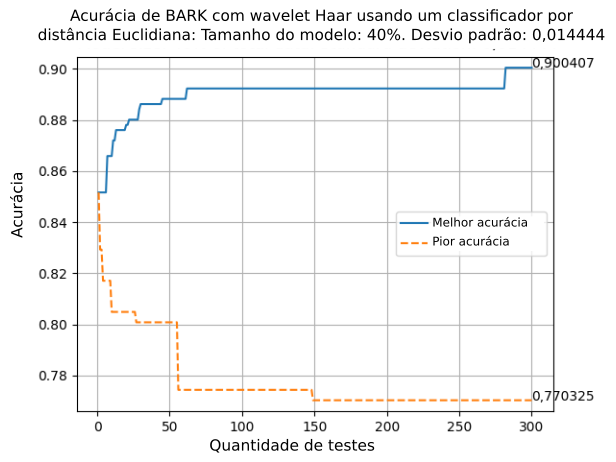
\includegraphics{images/results/confusionMatrices/classifier_Euclidian_40}
				\caption{Acurácia \textit{X} quantidade de testes - Distância Euclidiana, modelo a 40\%}
				\label{fig:classifiereuclidian40}
			\end{figure}
			\begin{table}[h]
\newcommand{\mc}[3]{\multicolumn{#1}{#2}{#3}}
\definecolor{tcB}{rgb}{0.447059,0.74902,0.266667}
\definecolor{tcC}{rgb}{0,0,0}
\definecolor{tcD}{rgb}{0,0.4,0.701961}
\definecolor{tcA}{rgb}{0.65098,0.65098,0.65098}
\begin{center}
	\begin{tabular}{ccc}
		% use packages: color,colortbl
		\mc{1}{l}{} & \mc{1}{>{\columncolor{tcA}}c}{\textbf{Verdadeiro}} & \mc{1}{>{\columncolor{tcA}}c}{\textbf{Falso}}\\

		\mc{1}{>{\columncolor{tcA}}r}{\textbf{Verdadeiro}} & \mc{1}{>{\columncolor{tcB}}c}{\textcolor{tcC}{233}} & \mc{1}{>{\columncolor{tcD}}c}{\textcolor{tcC}{35}}\\

		\mc{1}{>{\columncolor{tcA}}r}{\textbf{Falso}} & \mc{1}{>{\columncolor{tcD}}c}{\textcolor{tcC}{13}} & \mc{1}{>{\columncolor{tcB}}c}{\textcolor{tcC}{211}}
	\end{tabular}
	\caption{Tabela de confusão para classificador Euclidiano 40\%}
	\label{tab:classifier_Euclidian_40}
\end{center}
\end{table}

		
			\newpage
			\begin{figure}[h]
				\centering
				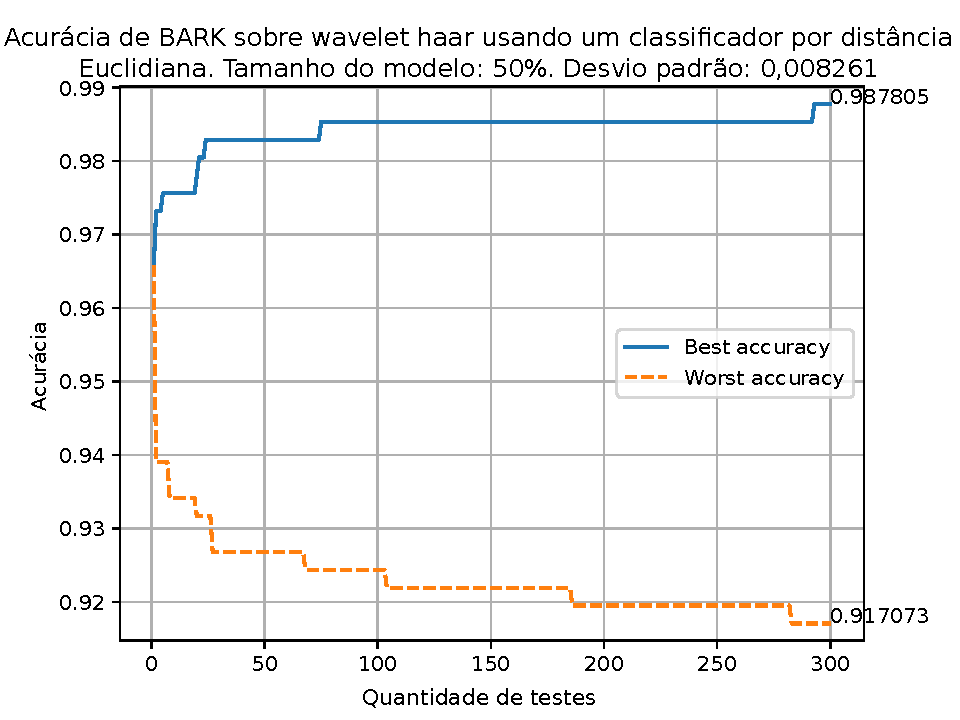
\includegraphics{images/results/confusionMatrices/classifier_Euclidian_50}
				\caption{Acurácia \textit{X} quantidade de testes - Distância Euclidiana, modelo a 50\%}
				\label{fig:classifiereuclidian50}
			\end{figure}
			\begin{table}[H]
	\newcommand{\mc}[3]{\multicolumn{#1}{#2}{#3}}
	\definecolor{tcB}{rgb}{0.447059,0.74902,0.266667}
	\definecolor{tcC}{rgb}{0,0,0}
	\definecolor{tcD}{rgb}{0,0.5,1}
	\definecolor{tcA}{rgb}{0.65098,0.65098,0.65098}
	\begin{center}
		\subfloat[Best matrix]{
			\begin{tabular}{ccc}
				% use packages: color,colortbl
				\mc{1}{l}{} & \mc{1}{>{\columncolor{tcA}}c}{\textbf{genuine}} & \mc{1}{>{\columncolor{tcA}}c}{\textbf{spoofed}}\\
				
				\mc{1}{>{\columncolor{tcA}}r}{\textbf{genuine}} & \mc{1}{>{\columncolor{tcB}}c}{\textcolor{tcC}{195}} & \mc{1}{>{\columncolor{tcD}}c}{\textcolor{tcC}{29}}\\
				
				\mc{1}{>{\columncolor{tcA}}r}{\textbf{spoofed}} & \mc{1}{>{\columncolor{tcD}}c}{\textcolor{tcC}{10}} & \mc{1}{>{\columncolor{tcB}}c}{\textcolor{tcC}{176}}
			\end{tabular}
			\label{tab:classifier_Euclidian_50_best}
		}
		\qquad
		\subfloat[Worst matrix]{
			\begin{tabular}{ccc}
				% use packages: color,colortbl
				\mc{1}{l}{} & \mc{1}{>{\columncolor{tcA}}c}{\textbf{genuine}} & \mc{1}{>{\columncolor{tcA}}c}{\textbf{spoofed}}\\
				
				\mc{1}{>{\columncolor{tcA}}r}{\textbf{genuine}} & \mc{1}{>{\columncolor{tcB}}c}{\textcolor{tcC}{193}} & \mc{1}{>{\columncolor{tcD}}c}{\textcolor{tcC}{79}}\\
				
				\mc{1}{>{\columncolor{tcA}}r}{\textbf{spoofed}} & \mc{1}{>{\columncolor{tcD}}c}{\textcolor{tcC}{12}} & \mc{1}{>{\columncolor{tcB}}c}{\textcolor{tcC}{126}}
			\end{tabular}
			\label{tab:classifier_Euclidian_50_worse}
		}
	\end{center}
	\caption{Confusion matrices for Euclidian distance classifier at 50\% model}
\end{table}
		
			\newpage
			\begin{figure}[h]
				\centering
				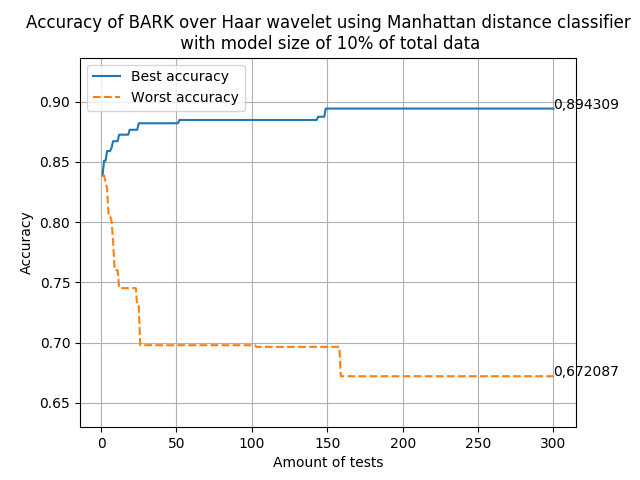
\includegraphics{images/results/confusionMatrices/classifier_Manhattan_10.png}
				\caption{Acurácia \textit{X} quantidade de testes - Distância Manhattan, modelo a 10\%}
				\label{fig:classifiermanhattan10}
			\end{figure}
			\begin{table}[h] 					\newcommand{\mc}[3]{\multicolumn{#1}{#2}{#3}} 					\definecolor{tcB}{rgb}{0.447059,0.74902,0.266667} 					\definecolor{tcC}{rgb}{0,0,0} 					\definecolor{tcD}{rgb}{0,0.5,1} 					\definecolor{tcA}{rgb}{0.65098,0.65098,0.65098} 					\begin{center} 						\subfloat[Melhor matriz de confusão]{ 							\begin{tabular}{ccc} 								\mc{1}{l}{} & \mc{1}{>{\columncolor{tcA}}c}{\textbf{genuíno}} & \mc{1}{>{\columncolor{tcA}}c}{\textbf{falsificado}}\\ 								\mc{1}{>{\columncolor{tcA}}r}{\textbf{genuíno}} & \mc{1}{>{\columncolor{tcB}}c}{\textcolor{tcC}{365}} & \mc{1}{>{\columncolor{tcD}}c}{\textcolor{tcC}{14}}\\ 								\mc{1}{>{\columncolor{tcA}}r}{\textbf{falsificado}} & \mc{1}{>{\columncolor{tcD}}c}{\textcolor{tcC}{4}} & \mc{1}{>{\columncolor{tcB}}c}{\textcolor{tcC}{355}} 							\end{tabular} 							\label{tab:classifier_Manhattan_10_best} 						} 						\qquad 						\subfloat[Pior matriz de confusão]{ 							\begin{tabular}{ccc} 								\mc{1}{l}{} & \mc{1}{>{\columncolor{tcA}}c}{\textbf{genuíno}} & \mc{1}{>{\columncolor{tcA}}c}{\textbf{falsificado}}\\ 								\mc{1}{>{\columncolor{tcA}}r}{\textbf{genuíno}} & \mc{1}{>{\columncolor{tcB}}c}{\textcolor{tcC}{289}} & \mc{1}{>{\columncolor{tcD}}c}{\textcolor{tcC}{11}}\\ 								\mc{1}{>{\columncolor{tcA}}r}{\textbf{falsificado}} & \mc{1}{>{\columncolor{tcD}}c}{\textcolor{tcC}{80}} & \mc{1}{>{\columncolor{tcB}}c}{\textcolor{tcC}{358}} 							\end{tabular} 							\label{tab:classifier_Manhattan_10_worse} 						} 					\end{center} 					\caption{Matrizes de confusão para distância Manhattan com modelo a 10\%} 				\end{table}
		
			\newpage
			\begin{figure}[h]
				\centering
				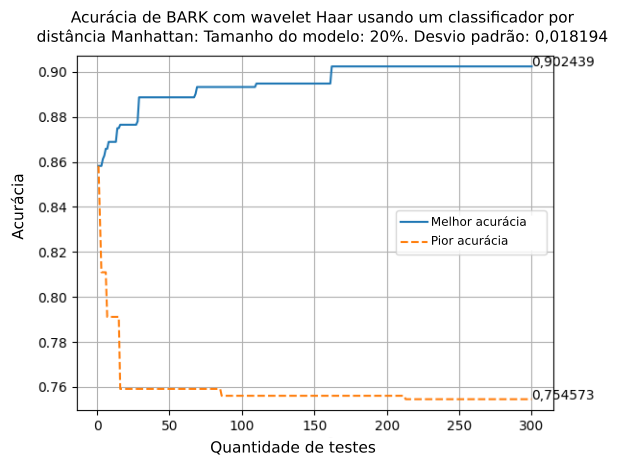
\includegraphics{images/results/confusionMatrices/classifier_Manhattan_20.png}
				\caption{Acurácia \textit{X} quantidade de testes - Distância Manhattan, modelo a 20\%}
				\label{fig:classifiermanhattan20}
			\end{figure}
			\begin{table}[h]
	\newcommand{\mc}[3]{\multicolumn{#1}{#2}{#3}}
	\definecolor{tcB}{rgb}{0.447059,0.74902,0.266667}
	\definecolor{tcC}{rgb}{0,0,0}
	\definecolor{tcD}{rgb}{0,0.5,1}
	\definecolor{tcA}{rgb}{0.65098,0.65098,0.65098}
	\begin{center}
		\subfloat[Melhor matriz]{
			\begin{tabular}{ccc}
				% use packages: color,colortbl
				\mc{1}{l}{} & \mc{1}{>{\columncolor{tcA}}c}{\textbf{Verdadeiro}} & \mc{1}{>{\columncolor{tcA}}c}{\textbf{Falso}}\\
				
				\mc{1}{>{\columncolor{tcA}}r}{\textbf{Verdadeiro}} & \mc{1}{>{\columncolor{tcB}}c}{\textcolor{tcC}{308}} & \mc{1}{>{\columncolor{tcD}}c}{\textcolor{tcC}{44}}\\
				
				\mc{1}{>{\columncolor{tcA}}r}{\textbf{Falso}} & \mc{1}{>{\columncolor{tcD}}c}{\textcolor{tcC}{20}} & \mc{1}{>{\columncolor{tcB}}c}{\textcolor{tcC}{284}}
			\end{tabular}
			\label{tab:classifier_Manhattan_20_best}
		}
		\qquad
		\subfloat[Pior matriz]{
			\begin{tabular}{ccc}
				% use packages: color,colortbl
				\mc{1}{l}{} & \mc{1}{>{\columncolor{tcA}}c}{\textbf{Verdadeiro}} & \mc{1}{>{\columncolor{tcA}}c}{\textbf{Falso}}\\
				
				\mc{1}{>{\columncolor{tcA}}r}{\textbf{Verdadeiro}} & \mc{1}{>{\columncolor{tcB}}c}{\textcolor{tcC}{316}} & \mc{1}{>{\columncolor{tcD}}c}{\textcolor{tcC}{149}}\\
				
				\mc{1}{>{\columncolor{tcA}}r}{\textbf{Falso}} & \mc{1}{>{\columncolor{tcD}}c}{\textcolor{tcC}{12}} & \mc{1}{>{\columncolor{tcB}}c}{\textcolor{tcC}{179}}
			\end{tabular}
			\label{tab:classifier_Manhattan_20_worst}
		}
	\end{center}
	\caption{Matrizes de confusão para o classificador por distâncias Manhattan com o uso de 20\% da base para modelagem}
\end{table}

	
			\newpage
			\begin{figure}[h]
				\centering
				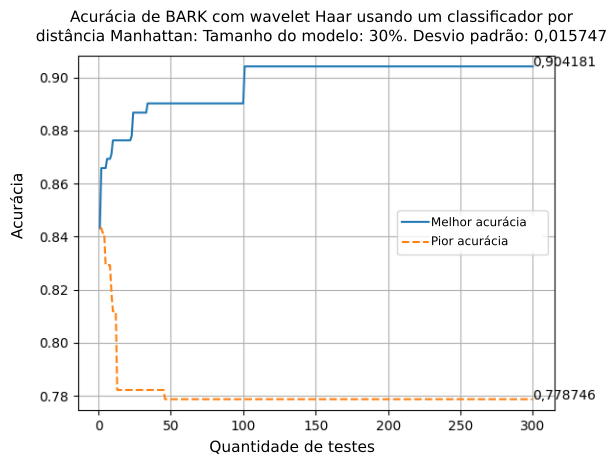
\includegraphics{images/results/confusionMatrices/classifier_Manhattan_30.png}
				\caption{Acurácia \textit{X} quantidade de testes - Distância Manhattan, modelo a 30\%}
				\label{fig:classifiermanhattan30}
			\end{figure}
			\begin{table}[h] 					\newcommand{\mc}[3]{\multicolumn{#1}{#2}{#3}} 					\definecolor{tcB}{rgb}{0.447059,0.74902,0.266667} 					\definecolor{tcC}{rgb}{0,0,0} 					\definecolor{tcD}{rgb}{0,0.5,1} 					\definecolor{tcA}{rgb}{0.65098,0.65098,0.65098} 					\begin{center} 						\subfloat[Melhor matriz de confusão]{ 							\begin{tabular}{ccc} 								\mc{1}{l}{} & \mc{1}{>{\columncolor{tcA}}c}{\textbf{genuíno}} & \mc{1}{>{\columncolor{tcA}}c}{\textbf{falsificado}}\\ 								\mc{1}{>{\columncolor{tcA}}r}{\textbf{genuíno}} & \mc{1}{>{\columncolor{tcB}}c}{\textcolor{tcC}{281}} & \mc{1}{>{\columncolor{tcD}}c}{\textcolor{tcC}{2}}\\ 								\mc{1}{>{\columncolor{tcA}}r}{\textbf{falsificado}} & \mc{1}{>{\columncolor{tcD}}c}{\textcolor{tcC}{6}} & \mc{1}{>{\columncolor{tcB}}c}{\textcolor{tcC}{285}} 							\end{tabular} 							\label{tab:classifier_Manhattan_30_best} 						} 						\qquad 						\subfloat[Pior matriz de confusão]{ 							\begin{tabular}{ccc} 								\mc{1}{l}{} & \mc{1}{>{\columncolor{tcA}}c}{\textbf{genuíno}} & \mc{1}{>{\columncolor{tcA}}c}{\textbf{falsificado}}\\ 								\mc{1}{>{\columncolor{tcA}}r}{\textbf{genuíno}} & \mc{1}{>{\columncolor{tcB}}c}{\textcolor{tcC}{256}} & \mc{1}{>{\columncolor{tcD}}c}{\textcolor{tcC}{19}}\\ 								\mc{1}{>{\columncolor{tcA}}r}{\textbf{falsificado}} & \mc{1}{>{\columncolor{tcD}}c}{\textcolor{tcC}{31}} & \mc{1}{>{\columncolor{tcB}}c}{\textcolor{tcC}{268}} 							\end{tabular} 							\label{tab:classifier_Manhattan_30_worse} 						} 					\end{center} 					\caption{Matrizes de confusão para distância Manhattan com modelo a 30\%} 				\end{table}
			
			\newpage
			\begin{figure}[h]
				\centering
				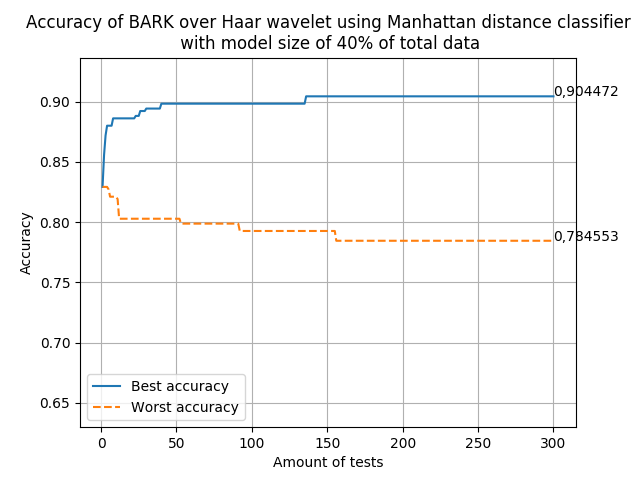
\includegraphics{images/results/confusionMatrices/classifier_Manhattan_40.png}
				\caption{Acurácia \textit{X} quantidade de testes - Distância Manhattan, modelo a 40\%}
				\label{fig:classifiermanhattan40}
			\end{figure}
			\begin{table}[h] 					\newcommand{\mc}[3]{\multicolumn{#1}{#2}{#3}} 					\definecolor{tcB}{rgb}{0.447059,0.74902,0.266667} 					\definecolor{tcC}{rgb}{0,0,0} 					\definecolor{tcD}{rgb}{0,0.5,1} 					\definecolor{tcA}{rgb}{0.65098,0.65098,0.65098} 					\begin{center} 						\subfloat[Best confusion matrix]{ 							\begin{tabular}{ccc} 								\mc{1}{l}{} & \mc{1}{>{\columncolor{tcA}}c}{\textbf{genuine}} & \mc{1}{>{\columncolor{tcA}}c}{\textbf{spoofed}}\\ 								\mc{1}{>{\columncolor{tcA}}r}{\textbf{genuine}} & \mc{1}{>{\columncolor{tcB}}c}{\textcolor{tcC}{244}} & \mc{1}{>{\columncolor{tcD}}c}{\textcolor{tcC}{5}}\\ 								\mc{1}{>{\columncolor{tcA}}r}{\textbf{spoofed}} & \mc{1}{>{\columncolor{tcD}}c}{\textcolor{tcC}{2}} & \mc{1}{>{\columncolor{tcB}}c}{\textcolor{tcC}{241}} 							\end{tabular} 							\label{tab:classifier_Manhattan_40_best} 						} 						\qquad 						\subfloat[Worst confusion matrix]{ 							\begin{tabular}{ccc} 								\mc{1}{l}{} & \mc{1}{>{\columncolor{tcA}}c}{\textbf{genuine}} & \mc{1}{>{\columncolor{tcA}}c}{\textbf{spoofed}}\\ 								\mc{1}{>{\columncolor{tcA}}r}{\textbf{genuine}} & \mc{1}{>{\columncolor{tcB}}c}{\textcolor{tcC}{218}} & \mc{1}{>{\columncolor{tcD}}c}{\textcolor{tcC}{7}}\\ 								\mc{1}{>{\columncolor{tcA}}r}{\textbf{spoofed}} & \mc{1}{>{\columncolor{tcD}}c}{\textcolor{tcC}{28}} & \mc{1}{>{\columncolor{tcB}}c}{\textcolor{tcC}{239}} 							\end{tabular} 							\label{tab:classifier_Manhattan_40_worse} 						} 					\end{center} 					\caption{Confusion matrices for Manhattan distance classifier at 40\% model} 				\end{table}
			
			\newpage
			\begin{figure}[h]
				\centering
				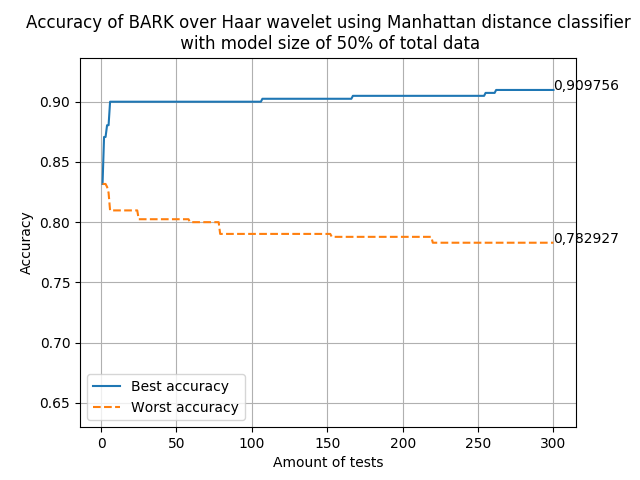
\includegraphics{images/results/confusionMatrices/classifier_Manhattan_50.png}
				\caption{Acurácia \textit{X} quantidade de testes - Distância Manhattan, modelo a 50\%}
				\label{fig:classifiermanhattan50}
			\end{figure}
			\begin{table}[h] 					\newcommand{\mc}[3]{\multicolumn{#1}{#2}{#3}} 					\definecolor{tcB}{rgb}{0.447059,0.74902,0.266667} 					\definecolor{tcC}{rgb}{0,0,0} 					\definecolor{tcD}{rgb}{0,0.5,1} 					\definecolor{tcA}{rgb}{0.65098,0.65098,0.65098} 					\begin{center} 						\subfloat[Best confusion matrix]{ 							\begin{tabular}{ccc} 								\mc{1}{l}{} & \mc{1}{>{\columncolor{tcA}}c}{\textbf{genuine}} & \mc{1}{>{\columncolor{tcA}}c}{\textbf{spoofed}}\\ 								\mc{1}{>{\columncolor{tcA}}r}{\textbf{genuine}} & \mc{1}{>{\columncolor{tcB}}c}{\textcolor{tcC}{172}} & \mc{1}{>{\columncolor{tcD}}c}{\textcolor{tcC}{30}}\\ 								\mc{1}{>{\columncolor{tcA}}r}{\textbf{spoofed}} & \mc{1}{>{\columncolor{tcD}}c}{\textcolor{tcC}{33}} & \mc{1}{>{\columncolor{tcB}}c}{\textcolor{tcC}{175}} 							\end{tabular} 							\label{tab:classifier_Manhattan_50_best} 						} 						\qquad 						\subfloat[Worst confusion matrix]{ 							\begin{tabular}{ccc} 								\mc{1}{l}{} & \mc{1}{>{\columncolor{tcA}}c}{\textbf{genuine}} & \mc{1}{>{\columncolor{tcA}}c}{\textbf{spoofed}}\\ 								\mc{1}{>{\columncolor{tcA}}r}{\textbf{genuine}} & \mc{1}{>{\columncolor{tcB}}c}{\textcolor{tcC}{142}} & \mc{1}{>{\columncolor{tcD}}c}{\textcolor{tcC}{58}}\\ 								\mc{1}{>{\columncolor{tcA}}r}{\textbf{spoofed}} & \mc{1}{>{\columncolor{tcD}}c}{\textcolor{tcC}{63}} & \mc{1}{>{\columncolor{tcB}}c}{\textcolor{tcC}{147}} 							\end{tabular} 							\label{tab:classifier_Manhattan_50_worse} 						} 					\end{center} 					\caption{Confusion matrices for Manhattan distance classifier at 50\% model} 				\end{table}
	
		\newpage
		\section{Experimento 03}
			\par Novamente, considerando que o experimento 1 teve como melhor resultado a combinação \textbf{Haar+BARK} o objetivo deste é constatar a máxima acurácia se consegue atingir em uma SVM. O dimensionamento do tamanho das amostras para o treinamento do classificador variou em 10\%, 20\%, 30\%, 40\% e finalmente 50\% do total das amostras. 300 foi a quantidade máxima de testes escolhida.
			
			\par Os resultados gerais são mostrados na tabela \ref{tab:experiment03Results}. 
			
			\par Mais níveis de detalhes podem ser consultados nas tabelas \ref{tab:classifier_SVM_10}, \ref{tab:classifier_Euclidian_20}, \ref{tab:classifier_SVM_30}, \ref{tab:classifier_Euclidian_40},  \ref{tab:classifier_SVM_50} e seus respectivos gráficos \ref{fig:classifiersvm10}, \ref{fig:classifiersvm20}, \ref{fig:classifiersvm30}, \ref{fig:classifiersvm40}, \ref{fig:classifiersvm50}.
	
			\begin{table}[H]
	\newcommand{\mc}[3]{\multicolumn{#1}{#2}{#3}}
	\definecolor{tcA}{rgb}{0.65098,0.65098,0.65098}
	\definecolor{tcB}{rgb}{0.447059,0.74902,0.266667}
	\begin{center}
		\caption{Resultados da abordagem com SVM}
		\begin{tabular}{|p{0.15\linewidth}|p{0.11\linewidth}|p{0.11\linewidth}|p{0.11\linewidth}|p{0.14\linewidth}|p{0.14\linewidth}|}\hline
			% use packages: color,colortbl
			\rowcolor{tcA}
			\centering\textbf{$M$} & \centering\textbf{Acurácia mínima} & \centering\textbf{Acurácia máxima} & \centering\textbf{Média das acurácias} & \centering\textbf{Desvio padrão da acurácia} & \begin{center}\textbf{EER}\end{center}\\\hline
			
			\rowcolor{tcB}
			% Loads data from tables/results/paraconsistentPlane/distParacomFrom10.csv
			\csvreader[
			late after line=\\\hline\rowcolor{tcB},%
			separator=comma,
			]{tables/results/experiment02ResultsSVM.csv}{1=\eme,2=\minAccu,3=\maxAccu,4=\meanAccu,5=\stdDev,6=\eer}{\centering\eme\% & \centering\StrSubstitute[0]{\minAccu}{.}{,} & \centering\StrSubstitute[0]{\maxAccu}{.}{,} & \centering\StrSubstitute[0]{\meanAccu}{.}{,} & \centering\StrSubstitute[0]{\stdDev}{.}{,} & \StrSubstitute[0]{\eer}{.}{,}}
			
		\end{tabular}
		\label{tab:experiment03Results}
		\\Fonte: Elaborado pelo autor, 2021.
	\end{center}
\end{table}
		
			\newpage
		\begin{figure}[h]
			\centering
			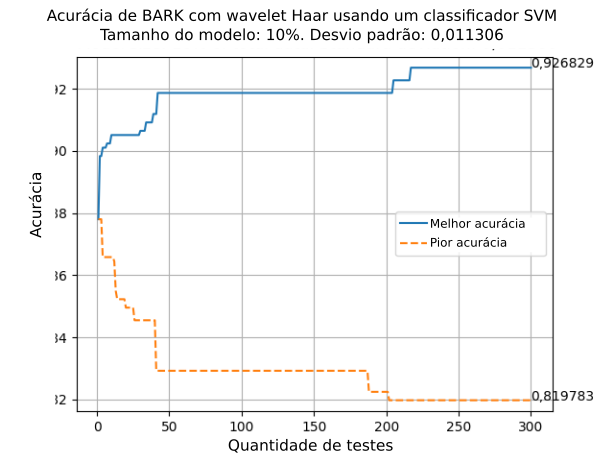
\includegraphics{images/results/confusionMatrices/classifier_SVM_10.png}
			\caption{Acurácia \textit{X} quantidade de testes - SVM, modelo a 10\%}
			\label{fig:classifiersvm10}
		\end{figure}
		\begin{table}[h]
\newcommand{\mc}[3]{\multicolumn{#1}{#2}{#3}}
\definecolor{tcB}{rgb}{0.447059,0.74902,0.266667}
\definecolor{tcC}{rgb}{0,0,0}
\definecolor{tcD}{rgb}{0,0.4,0.701961}
\definecolor{tcA}{rgb}{0.65098,0.65098,0.65098}
\begin{center}
	\begin{tabular}{ccc}
		% use packages: color,colortbl
		\mc{1}{l}{} & \mc{1}{>{\columncolor{tcA}}c}{\textbf{Verdadeiro}} & \mc{1}{>{\columncolor{tcA}}c}{\textbf{Falso}}\\

		\mc{1}{>{\columncolor{tcA}}r}{\textbf{Verdadeiro}} & \mc{1}{>{\columncolor{tcB}}c}{\textcolor{tcC}{339}} & \mc{1}{>{\columncolor{tcD}}c}{\textcolor{tcC}{24}}\\

		\mc{1}{>{\columncolor{tcA}}r}{\textbf{Falso}} & \mc{1}{>{\columncolor{tcD}}c}{\textcolor{tcC}{30}} & \mc{1}{>{\columncolor{tcB}}c}{\textcolor{tcC}{345}}
	\end{tabular}
	\caption{Melhor tabela de confusão para classificador SVM 10\%}
	\label{tab:classifier_SVM_10_best}
\end{center}
\end{table}

\begin{table}[h]
	\newcommand{\mc}[3]{\multicolumn{#1}{#2}{#3}}
	\definecolor{tcB}{rgb}{0.447059,0.74902,0.266667}
	\definecolor{tcC}{rgb}{0,0,0}
	\definecolor{tcD}{rgb}{0,0.4,0.701961}
	\definecolor{tcA}{rgb}{0.65098,0.65098,0.65098}
	\begin{center}
		\begin{tabular}{ccc}
			% use packages: color,colortbl
			\mc{1}{l}{} & \mc{1}{>{\columncolor{tcA}}c}{\textbf{Verdadeiro}} & \mc{1}{>{\columncolor{tcA}}c}{\textbf{Falso}}\\
			
			\mc{1}{>{\columncolor{tcA}}r}{\textbf{Verdadeiro}} & \mc{1}{>{\columncolor{tcB}}c}{\textcolor{tcC}{329}} & \mc{1}{>{\columncolor{tcD}}c}{\textcolor{tcC}{93}}\\
			
			\mc{1}{>{\columncolor{tcA}}r}{\textbf{Falso}} & \mc{1}{>{\columncolor{tcD}}c}{\textcolor{tcC}{40}} & \mc{1}{>{\columncolor{tcB}}c}{\textcolor{tcC}{276}}
		\end{tabular}
		\caption{Pior tabela de confusão para classificador SVM 10\%}
		\label{tab:classifier_SVM_10_worse}
	\end{center}
\end{table}

	
		\newpage
		\begin{figure}[h]
			\centering
			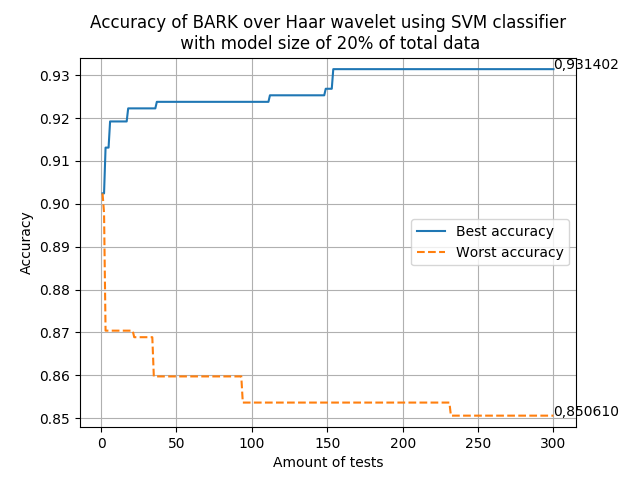
\includegraphics{images/results/confusionMatrices/classifier_SVM_20.png}
			\caption{Acurácia \textit{X} quantidade de testes - SVM, modelo a 20\%}
			\label{fig:classifiersvm20}
		\end{figure}
		\begin{table}[h] 					\newcommand{\mc}[3]{\multicolumn{#1}{#2}{#3}} 					\definecolor{tcB}{rgb}{0.447059,0.74902,0.266667} 					\definecolor{tcC}{rgb}{0,0,0} 					\definecolor{tcD}{rgb}{0,0.5,1} 					\definecolor{tcA}{rgb}{0.65098,0.65098,0.65098} 					\begin{center} 						\subfloat[Best confusion matrix]{ 							\begin{tabular}{ccc} 								\mc{1}{l}{} & \mc{1}{>{\columncolor{tcA}}c}{\textbf{genuine}} & \mc{1}{>{\columncolor{tcA}}c}{\textbf{spoofed}}\\ 								\mc{1}{>{\columncolor{tcA}}r}{\textbf{genuine}} & \mc{1}{>{\columncolor{tcB}}c}{\textcolor{tcC}{306}} & \mc{1}{>{\columncolor{tcD}}c}{\textcolor{tcC}{29}}\\ 								\mc{1}{>{\columncolor{tcA}}r}{\textbf{spoofed}} & \mc{1}{>{\columncolor{tcD}}c}{\textcolor{tcC}{22}} & \mc{1}{>{\columncolor{tcB}}c}{\textcolor{tcC}{299}} 							\end{tabular} 							\label{tab:classifier_Euclidian_10_best} 						} 						\qquad 						\subfloat[Worst confusion matrix]{ 							\begin{tabular}{ccc} 								\mc{1}{l}{} & \mc{1}{>{\columncolor{tcA}}c}{\textbf{genuine}} & \mc{1}{>{\columncolor{tcA}}c}{\textbf{spoofed}}\\ 								\mc{1}{>{\columncolor{tcA}}r}{\textbf{genuine}} & \mc{1}{>{\columncolor{tcB}}c}{\textcolor{tcC}{255}} & \mc{1}{>{\columncolor{tcD}}c}{\textcolor{tcC}{56}}\\ 								\mc{1}{>{\columncolor{tcA}}r}{\textbf{spoofed}} & \mc{1}{>{\columncolor{tcD}}c}{\textcolor{tcC}{73}} & \mc{1}{>{\columncolor{tcB}}c}{\textcolor{tcC}{272}} 							\end{tabular} 							\label{tab:classifier_Euclidian_10_worse} 						} 					\end{center} 					\caption{Confusion matrices for SVM classifier at 20\% model} 				\end{table}
		
		\newpage
		\begin{figure}[h]
			\centering
			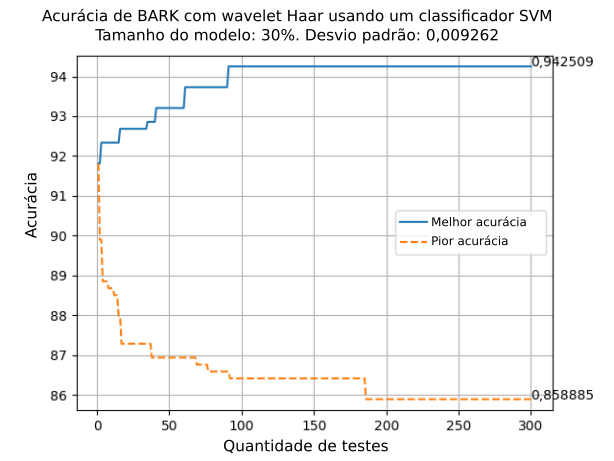
\includegraphics{images/results/confusionMatrices/classifier_SVM_30.png}
			\caption{Acurácia \textit{X} quantidade de testes - SVM, modelo a 30\%}
			\label{fig:classifiersvm30}
		\end{figure}
		\begin{table}[h] 					\newcommand{\mc}[3]{\multicolumn{#1}{#2}{#3}} 					\definecolor{tcB}{rgb}{0.447059,0.74902,0.266667} 					\definecolor{tcC}{rgb}{0,0,0} 					\definecolor{tcD}{rgb}{0,0.5,1} 					\definecolor{tcA}{rgb}{0.65098,0.65098,0.65098} 					\begin{center} 						\subfloat[Best confusion matrix]{ 							\begin{tabular}{ccc} 								\mc{1}{l}{} & \mc{1}{>{\columncolor{tcA}}c}{\textbf{genuine}} & \mc{1}{>{\columncolor{tcA}}c}{\textbf{spoofed}}\\ 								\mc{1}{>{\columncolor{tcA}}r}{\textbf{genuine}} & \mc{1}{>{\columncolor{tcB}}c}{\textcolor{tcC}{272}} & \mc{1}{>{\columncolor{tcD}}c}{\textcolor{tcC}{27}}\\ 								\mc{1}{>{\columncolor{tcA}}r}{\textbf{spoofed}} & \mc{1}{>{\columncolor{tcD}}c}{\textcolor{tcC}{15}} & \mc{1}{>{\columncolor{tcB}}c}{\textcolor{tcC}{260}} 							\end{tabular} 							\label{tab:classifier_Euclidian_10_best} 						} 						\qquad 						\subfloat[Worst confusion matrix]{ 							\begin{tabular}{ccc} 								\mc{1}{l}{} & \mc{1}{>{\columncolor{tcA}}c}{\textbf{genuine}} & \mc{1}{>{\columncolor{tcA}}c}{\textbf{spoofed}}\\ 								\mc{1}{>{\columncolor{tcA}}r}{\textbf{genuine}} & \mc{1}{>{\columncolor{tcB}}c}{\textcolor{tcC}{233}} & \mc{1}{>{\columncolor{tcD}}c}{\textcolor{tcC}{39}}\\ 								\mc{1}{>{\columncolor{tcA}}r}{\textbf{spoofed}} & \mc{1}{>{\columncolor{tcD}}c}{\textcolor{tcC}{54}} & \mc{1}{>{\columncolor{tcB}}c}{\textcolor{tcC}{248}} 							\end{tabular} 							\label{tab:classifier_Euclidian_10_worse} 						} 					\end{center} 					\caption{Confusion matrices for SVM classifier at 30\% model} 				\end{table}
	
		\newpage
		\begin{figure}[h]
			\centering
			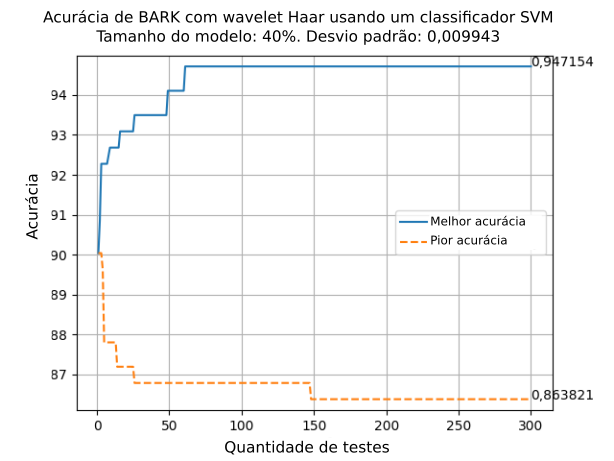
\includegraphics{images/results/confusionMatrices/classifier_SVM_40.png}
			\caption{Acurácia \textit{X} quantidade de testes - SVM, modelo a 40\%}
			\label{fig:classifiersvm40}
		\end{figure}
		\begin{table}[h]
\newcommand{\mc}[3]{\multicolumn{#1}{#2}{#3}}
\definecolor{tcB}{rgb}{0.447059,0.74902,0.266667}
\definecolor{tcC}{rgb}{0,0,0}
\definecolor{tcD}{rgb}{0,0.5,1}
\definecolor{tcA}{rgb}{0.65098,0.65098,0.65098}
\begin{center}
	\begin{tabular}{ccc}
		% use packages: color,colortbl
		\mc{1}{l}{} & \mc{1}{>{\columncolor{tcA}}c}{\textbf{Verdadeiro}} & \mc{1}{>{\columncolor{tcA}}c}{\textbf{Falso}}\\

		\mc{1}{>{\columncolor{tcA}}r}{\textbf{Verdadeiro}} & \mc{1}{>{\columncolor{tcB}}c}{\textcolor{tcC}{234}} & \mc{1}{>{\columncolor{tcD}}c}{\textcolor{tcC}{14}}\\

		\mc{1}{>{\columncolor{tcA}}r}{\textbf{Falso}} & \mc{1}{>{\columncolor{tcD}}c}{\textcolor{tcC}{12}} & \mc{1}{>{\columncolor{tcB}}c}{\textcolor{tcC}{232}}
	\end{tabular}
	\caption{Melhor tabela de confusão para classificador SVM 40\%}
	\label{tab:classifier_SVM_40_best}
\end{center}
\end{table}

\begin{table}[h]
	\newcommand{\mc}[3]{\multicolumn{#1}{#2}{#3}}
	\definecolor{tcB}{rgb}{0.447059,0.74902,0.266667}
	\definecolor{tcC}{rgb}{0,0,0}
	\definecolor{tcD}{rgb}{0,0.5,1}
	\definecolor{tcA}{rgb}{0.65098,0.65098,0.65098}
	\begin{center}
		\begin{tabular}{ccc}
			% use packages: color,colortbl
			\mc{1}{l}{} & \mc{1}{>{\columncolor{tcA}}c}{\textbf{Verdadeiro}} & \mc{1}{>{\columncolor{tcA}}c}{\textbf{Falso}}\\
			
			\mc{1}{>{\columncolor{tcA}}r}{\textbf{Verdadeiro}} & \mc{1}{>{\columncolor{tcB}}c}{\textcolor{tcC}{216}} & \mc{1}{>{\columncolor{tcD}}c}{\textcolor{tcC}{37}}\\
			
			\mc{1}{>{\columncolor{tcA}}r}{\textbf{Falso}} & \mc{1}{>{\columncolor{tcD}}c}{\textcolor{tcC}{30}} & \mc{1}{>{\columncolor{tcB}}c}{\textcolor{tcC}{209}}
		\end{tabular}
		\caption{Pior tabela de confusão para classificador SVM 40\%}
		\label{tab:classifier_SVM_40_worse}
	\end{center}
\end{table}

	
		\newpage
		\begin{figure}[h]
			\centering
			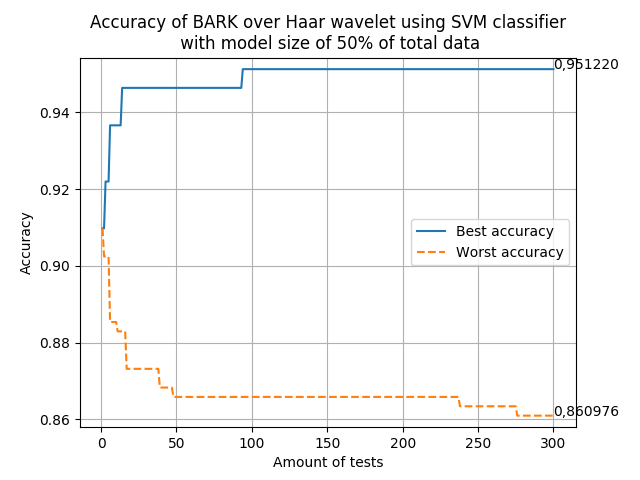
\includegraphics{images/results/confusionMatrices/classifier_SVM_50.png}
			\caption{Acurácia \textit{X} quantidade de testes - SVM, modelo a 50\%}
			\label{fig:classifiersvm50}
		\end{figure}
		\begin{table}[h] 					\newcommand{\mc}[3]{\multicolumn{#1}{#2}{#3}} 					\definecolor{tcB}{rgb}{0.447059,0.74902,0.266667} 					\definecolor{tcC}{rgb}{0,0,0} 					\definecolor{tcD}{rgb}{0,0.5,1} 					\definecolor{tcA}{rgb}{0.65098,0.65098,0.65098} 					\begin{center} 						\subfloat[Best confusion matrix]{ 							\begin{tabular}{ccc} 								\mc{1}{l}{} & \mc{1}{>{\columncolor{tcA}}c}{\textbf{genuine}} & \mc{1}{>{\columncolor{tcA}}c}{\textbf{spoofed}}\\ 								\mc{1}{>{\columncolor{tcA}}r}{\textbf{genuine}} & \mc{1}{>{\columncolor{tcB}}c}{\textcolor{tcC}{205}} & \mc{1}{>{\columncolor{tcD}}c}{\textcolor{tcC}{1}}\\ 								\mc{1}{>{\columncolor{tcA}}r}{\textbf{spoofed}} & \mc{1}{>{\columncolor{tcD}}c}{\textcolor{tcC}{0}} & \mc{1}{>{\columncolor{tcB}}c}{\textcolor{tcC}{204}} 							\end{tabular} 							\label{tab:classifier_SVM_50_best} 						} 						\qquad 						\subfloat[Worst confusion matrix]{ 							\begin{tabular}{ccc} 								\mc{1}{l}{} & \mc{1}{>{\columncolor{tcA}}c}{\textbf{genuine}} & \mc{1}{>{\columncolor{tcA}}c}{\textbf{spoofed}}\\ 								\mc{1}{>{\columncolor{tcA}}r}{\textbf{genuine}} & \mc{1}{>{\columncolor{tcB}}c}{\textcolor{tcC}{196}} & \mc{1}{>{\columncolor{tcD}}c}{\textcolor{tcC}{17}}\\ 								\mc{1}{>{\columncolor{tcA}}r}{\textbf{spoofed}} & \mc{1}{>{\columncolor{tcD}}c}{\textcolor{tcC}{9}} & \mc{1}{>{\columncolor{tcB}}c}{\textcolor{tcC}{188}} 							\end{tabular} 							\label{tab:classifier_SVM_50_worse} 						} 					\end{center} 					\caption{Confusion matrices for SVM distance classifier at 50\% model} 				\end{table}
	
	\newpage
	\section{Experimento 04}
		\par Os experimentos \ref{chap:propApproach:sec:Experimento01}, \ref{chap:propApproach:sec:Experimento02}, \ref{chap:propApproach:sec:Experimento03} mostraram que a combinação \textbf{\textit{wavelet haar + escala BARK}} é a melhor para geração de vetores de características e que esses possibilitam classificações razoáveis com classificadores simples. Esse experimento visa responder, qual o motivo dessa combinação funcionar melhor.
		\par As \textit{wavelets} \textbf{haar} e \textbf{daubechies 42} conseguiram respectivamente os melhores e os piores vetores de características na escala \textit{BARK}. Já em \textit{MEL}, \textbf{haar} foi a melhor e \textbf{daubechies 54} a pior.
		\par Para fins comparativos, foi criado um sinal periódico sobre o qual serão aplicadas as transformadas \textit{wavelet} correspondentes aos melhores e piores desempenhos, os resultados dessa aplicação, assim como o sinal original, constituem o gráfico mostrado na figura \ref{fig:haardaub42comparison}.
		\par O sinal periódico foi construído com a sequência \textit{32, 10, 20, 38, 37, 28, 38, 34, 18, 24, 24, 9, 23, 24, 28, 34} repetida 32 vezes.
		\par No gráfico supracitado o sinal de controle é periódico e contém 512 posições, portanto, considerando a abordagem de decomposição máxima, foram aplicadas as transformadas \textit{wavelet packet} até o nível 8.
		
		\begin{figure}[h]
			\centering
			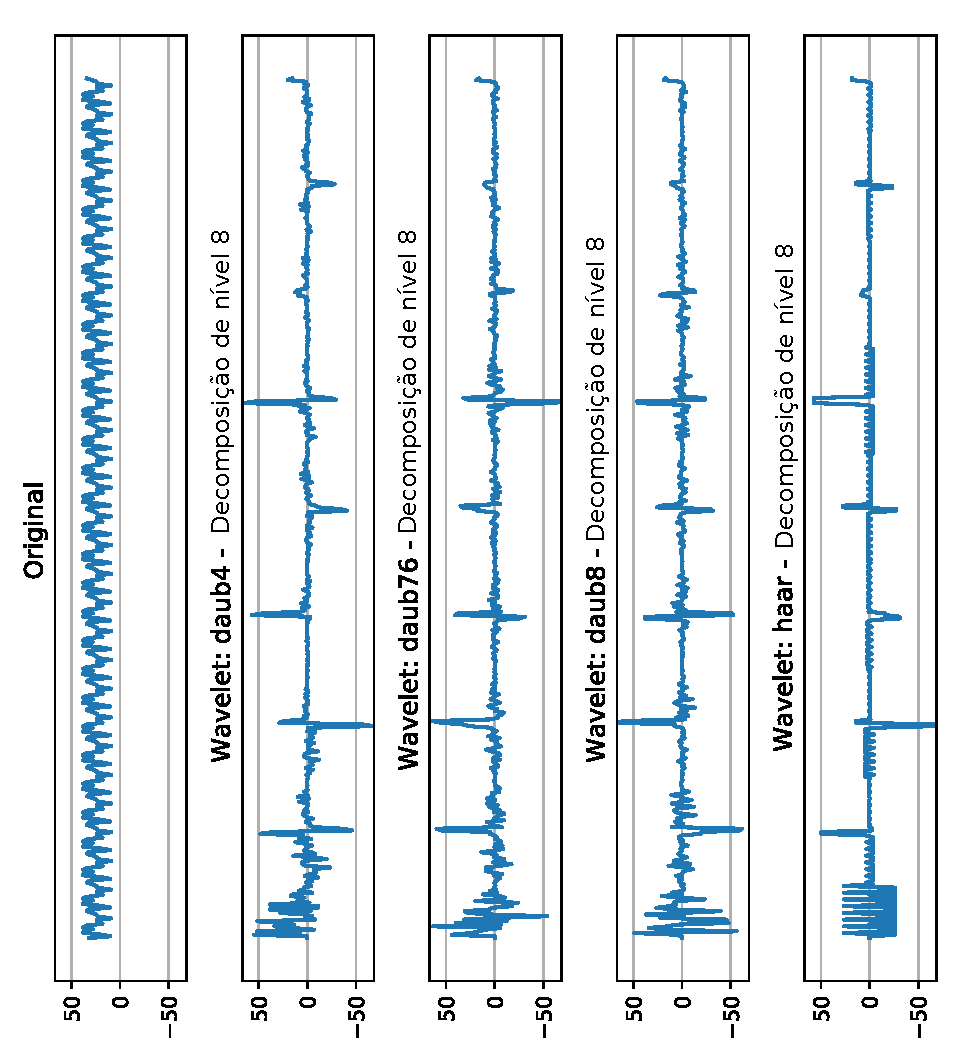
\includegraphics[width=0.6\linewidth]{images/results/haarDaubComparison/haarDaub42Comparison.pdf}
			\caption{Comparação wavelets \textit{haar} e \textit{daubechies 42, 54}}
			\label{fig:haardaub42comparison}
		\end{figure}
		
		\par É possível perceber que a separação das componentes do sinal é muito melhor delimitada na \textit{wavelet haar} do que na mesma transformação com a \textit{daubechies 42 e 54}, gerando assim um sinal mais separável, para ser lido tanto segundo a escala \textit{BARK} como \textit{MEL}.
		

	